\subsection{Data Acquisition}

The primary data manipulated in this study are university course syllabi.
Currently the experimental data include documents obtained from the George
Mason University departments of Computer Science and Statistics as well as
the Portland State University department of Computer Science. Simple web
scrapers were written using Python and BeautifulSoup to download publicly
available syllabi from departmental web pages. Syllabi occurred in a number
of different formats, most commonly HTML, Portable Document Format,
Microsoft Word Documents, and Rich Text Format. A parser was written for
each of these formats to acquire the contained, unstructured text, which
was then passed through a cleaning procedure to remove abbreviations and
non-English characters.

The Python scraping framework employed is structured to allow pluggable web
scrapers tooled to specific syllabus repositories. A major future goal is
to expand the breadth of data collection across different institutions.
Development is in progress for new scraping engines tooled to new
repositories.

%------------------------------------------------

\subsection{Preliminary Data Exploration}

Preliminary exploratory results are promising. We applied K-Means
clustering to a sample dataset of syllabi scraped from the GMU Computer
Science online archive of syllabi. Using course sections across semesters
as ground-truth labels, we obtained results summarized in
\tref{table:cluster-metrics} and \tref{table:cluster-results}. A
distributed implementation of K-Means available in the Python toolkit
\texttt{scikit-learn} was used to perform the clustering.

The high completeness values are promising: this indicates that many of the
same course are assigned under the same cluster prototype. The low value of
homogeneity is unsurprising given the initialization parameters used:
K-Means was forced to detect only 20 clusters, a far smaller number than
the magnitude of distinct course sections available. The number 20 was
chosen arbitrarily as a smaller count than the true number of distinct
course sections in order to increase cluster size. Cursory visual
inspection of the most common frequencies in the first few clusters
(\tref{table:cluster-results}) also supports the structured nature of the
dataset with semantically related terms grouped together in a logical
fashion corresponding with an obvious, known GMU course.

\begin{table}[ht]
\centering
\makebox[0pt][c]{\parbox{1.2\textwidth}{%
  \begin{minipage}[ht]{0.40\hsize}\centering
    \begin{tabular}{ll}
    \toprule
    Execution time & 0.144568s \\
    Homogeneity & 0.415 \\
    Completeness & 0.877 \\
    V-measure & 0.563 \\
    \bottomrule
    \end{tabular}
    \caption{Preliminary clustering metrics\label{table:cluster-metrics}}
  \end{minipage}
  \hfill
  \begin{minipage}[ht]{0.56\hsize}\centering
    \begin{tabular}{lll}
    \toprule
    Cluster 1 &
    Cluster 2 &
    Cluster 3 \\
    \midrule
    intelligence & chapter      & software \\
    artificial   & project      & swe \\
    agents       & sipser       & testing \\
    learning     & networks     & web \\
    tecuci       & layer        & interfaces \\
    expert       & savitch      & construction \\
    knowledge    & data         & design \\
    reasoning    & dlc          & constructing \\
    semantic     & experimental & professor \\
    intelligent  & design       & quality \\
    \bottomrule
    \end{tabular}
    \caption{Structure of clustering results\label{table:cluster-results}}
  \end{minipage}
}}
\end{table}

%------------------------------------------------

\subsection{Topic Modeling}

After the exploratory clustering process, we passed cleaned data into a
topic modeling framework. The Java MALLET library is used to perform
\acf{lda} on the combined syllabus data set. A data pipeline is
constructed using the MALLET API that reads input data, tokenizes it,
strips stop words, and trains an \ac{lda} topic model. Initial topic
modeling results are later piped into a simple, interactive user interface.

Sample preliminary results are illustrated in \tref{table:ldadocs}, showing
the breakdown of documents into component topics, and
\tref{table:ldatopics}, showing topic definition.  Further study is needed
to evaluate the success of this method and its application to the data set.
Additionally, further work is needed to construct labels for the data set.
That is, each course syllabus is currently an anonymous, independent data
point. No metadata is considered, specifically semester or section name.


\begin{table}[ht]
\centering
\begin{tabular}{lllll}
\toprule
Doc & Topic & Proportion & Topic & Proportion \\
\midrule
0 & 33 & 0.7666641741676518 & 62 & 0.230550274742815 \\
1 & 44 & 0.5776374037067855 & 8  & 0.3152509716025131 \\
2 & 86 & 0.8143297134325639 & 62 & 0.18015768047706127 \\
3 & 9  & 0.9491106700671812 & 5  & 0.034876914241398584 \\
4 & 82 & 0.5736690412365056 & 53 & 0.39539480434234386 \\
\bottomrule
\end{tabular}
\caption{Structure of per-document topic breakdown\label{table:ldadocs}}
\end{table}


\begin{table}[ht]
\centering
\begin{tabular}{lllll}
\toprule
Topic & Term & Term & Term & Term \\
\midrule
0 & lisp (98)          & june (57)        & prolog (46)    & http (45) \\
1 & systems (154)      & operating (119)  & system (101)   & programming (92) \\
2 & systems (304)      & operating (252)  & students (189) & projects (146) \\
3 & randomization (66) & trials (57)      & clinical (57)  & outcome (30) \\
4 & database (389)     & relational (151) & design (133)   & model (124) \\
\bottomrule
\end{tabular}
\caption{Structure of topic term-frequency definition\label{table:ldatopics}}
\end{table}


%------------------------------------------------

\subsection{Visualization}

A basic, interactive user visualization of syllabus topics has been
prototyped. Output data is piped from the topic model and stored a simple
relational database to store topic definitions and document composition
information. This data is then combinatorially expanded into two
cross-referenced HTML documents using a simple Python script. Images of the
visualization are included for reference, see \fref{fig:vis-docs} and
\fref{fig:vis-topics}. It will be a subject of future work to create a
richer browsing experience to investigate learned document topics.

\begin{figure}[ht]
\centering
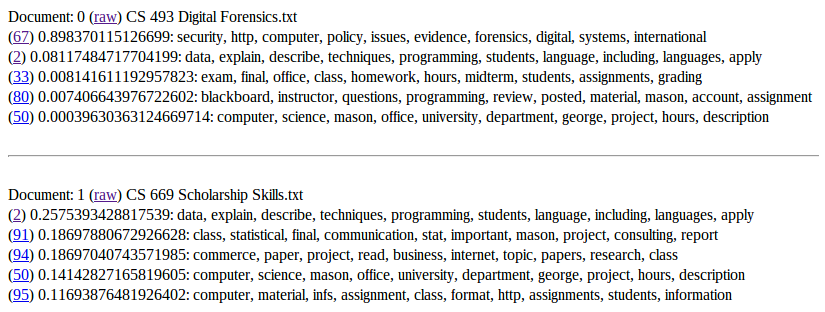
\includegraphics[width=0.98\textwidth]{figures/vis-docs.png}
\caption{Per-document topic breakdown\label{fig:vis-docs}}
\end{figure}

\begin{figure}[ht]
\centering
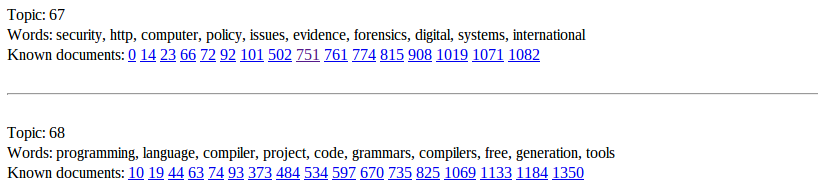
\includegraphics[width=0.98\textwidth]{figures/vis-topics.png}
\caption{Topic-word definitions\label{fig:vis-topics}}
\end{figure}

%------------------------------------------------

\subsection{Evaluation}

Results evaluation will require two components: the generation of predicted
topics and a set of known-good, reliable benchmark topics. The benchmark
topics can be classified ``known-good'' if they encode domain expertise, a
characteristic which is fundamentally lacking from the unsupervised topic
modeling process. Once a set of proposed topics is obtained from the
syllabus data set, the known-good categorization of concepts with labels
will be used to propose a second set of topics.  Overlap between these two
groups of topics will be used to share labels from the known-good set to
the experimentally proposed group with some value of confidence. Those
common topics will be strongly endorsed or validated, while outliers may be
trimmed if under a certain confidence threshold.

External parties occasionally maintain detailed descriptions of
expectations for specific hypothetical courses. For example the ACM
maintains an annual writeup of guidelines for undergraduate education.
\cite{CS2013} These course descriptions could be employed as the secondary
corpus to include implicit expert knowledge.

%------------------------------------------------

\subsection{Resources}

The primary software libraries employed to support this project are the
Python machine learning toolkit
\texttt{scikit-learn}\footnote{\url{http://scikit-learn.org}}, the Java
toolkit \texttt{Mallet}\footnote{\url{http://mallet.cs.umass.edu}}, and the
Python web scraping library
BeautifulSoup\footnote{\url{http://www.crummy.com/software/BeautifulSoup/}}.
Other libraries may be incorporated as needed.

Syllabus data has been collected from the George Mason University
departments of Computer Science\footnote{\url{http://cs.gmu.edu/courses/}}
and Statistics\footnote{\url{http://statistics.gmu.edu/courses/}} along
with the Portland State University department of computer
Science\footnote{\url{http://www.pdx.edu/computer-science/courses}}.
Additional institutions targeted for future scraping include Colorado,
Rice, UNCG, and Chaminade. All of the listed schools host publicly
available syllabus archives, at least for some departments. It may become
necessary to contact other universities directly to acquire their syllabus
data. Additionally, the Open Syllabus
Project\footnote{\url{http://opensyllabusproject.org}} may prove a useful
resource or collaborator in the future.

%------------------------------------------------
